The goal of this chapter is to discuss the performance of Bacco, using a variety of parameters, methods, and laboratory
tests. The results will also be compared to the ones obtained by applying the same procedures to devices using the
LoRaWAN protocol.

\section{Time On Air And Duty Cycle}
\Gls{ToA} is a crucial metric to take into consideration when measuring the performance of a network protocol. It is
defined as the time that a device takes to transmit a packet on the channel. At the same conditions, a shorter \gls{ToA}
results in improved energy efficiency and a smaller probability of interference with packets transmitted from other
devices.\\
\Gls{ToA} is correlated to the packet length in symbols (a longer packet will require a longer transmission time).
Referencing the official LoRa documentation, see \cite{sx1262}, we can find that \gls{ToA} is
discussed in section 6.1.4; in particular the exact formula for \gls{ToA} is shown here by Equation \ref{eqn: ToA}.
\begin{equation}
    \label{eqn: ToA}
    \mathit{ToA} = \frac{2^{\mathit{SF}}}{\mathit{BW}}*\mathit{N_{symbols}}
\end{equation}
where
\begin{itemize}[noitemsep,nolistsep]
    \item[\boldmath$\cdot$] $\mathit{SF}$ is the Spreading Factor (from 5 to 12);
    \item[\boldmath$\cdot$] $\mathit{BW}$ is the Bandwidth (in kHz);
    \item[\boldmath$\cdot$] $\mathit{N_{symbols}}$ is the number of symbols in the packet.
\end{itemize}
\vspace{0.55cm}
$\mathit{N_{symbols}}$ can be calculated knowing the number of bytes that compose the packet ($\mathit{N_{bytes_{payload}}}
$) by using Equation \ref{eqn: n_symbols}.

\begin{equation}
    \label{eqn: n_symbols}
    \resizebox{.9\hsize}{!}{
        \ensuremath{
            \mathit{N_{symbols}} = \mathit{N_{symbols_{preamble}}} + 12.25 + \textit{max} \left( \textit{ceil} \left(
                    \frac{8 * \mathit{N_{bytes_{MAC}}} - 4 * \mathit{SF} + 24 + 20 * H}{4 * \mathit{SF}} \right), 0 \right) * \frac{4}{\mathit{CR}}}}
\end{equation}

where
\begin{itemize}[noitemsep,nolistsep]
    \item[\boldmath$\cdot$] $\mathit{N_{symbols_{preamble}}}$ is equal to the number of symbols in the preamble sync message.
        This parameter can be set arbitrarily, but it is often given a value of 8.
    \item[\boldmath$\cdot$] $H$ denotes the presence of an explicit physical layer header. It assumes the
        value of 1 when the header is present and 0 when it is not present;
    \item[\boldmath$\cdot$] $\mathit{CR}$ is equal to the coding rate. It can be set to $\frac{4}{5},\frac{4}{6},
        \frac{4}{7}$ or $\frac{4}{8}$.
    \item[\boldmath$\cdot$] $\mathit{N_{bytes_{MAC}}}$ is equal to the total number of bytes of the \gls{MAC} packet.
\end{itemize}
\vspace{0.55cm}
The duty cycle is the fraction of time in which the channel is busy, it can be calculated using Equation \ref{eqn: duty cycle}.
\begin{equation}
    \label{eqn: duty cycle}
    d = \frac{\tau}{T}
\end{equation}
where
\begin{itemize}[noitemsep,nolistsep]
    \item[\boldmath$\cdot$] $d$ is the duty cycle;
    \item[\boldmath$\cdot$] $\tau$ is the \gls{ToA};
    \item[\boldmath$\cdot$] $T$ is the transmission period.
\end{itemize}


\subsection{Regulations}
\label{subsec: regulations}
To ensure a fair distribution of the transmission activity, local, national and international governments
define limits on the usage of the radio channel. The limits vary by the frequency band in which the devices operate.
The two parameters that are often used as an upper bound not to be crossed are \gls{ERP}\footnote{\gls{ERP} is the
measure of the power effectively radiated by an antenna system in a specific direction, accounting for both transmitter
output and antenna characteristic. It is commonly expressed in watts or decibels and it is used for determining the coverage area
and range of a radio.} and duty cycle.\\
Using the current Italian regulations at the time of writing as an example, we can observe that the spectrum is split into
frequency bands that can be either free, reserved, or restricted; each of them has three parameters associated with it: the
maximum \gls{ERP}, the minimum channel bandwidth and the maximum duty cycle. The official document
that discusses this matter in detail can be found in \cite{gazzetta_potenza_868}. The bands that LoRa devices use in
Europe are $\[868.0,868.6\]$ MHz and $\[868.7,869.2\]$ MHz, they both feature a maximum \gls{ERP} of 25 mW or 14 dBm and
do not have any restriction on channel bandwidth, however, the first band has a maximum duty cycle of 1\%, while for the
other the limit is set to 0.1\%.\\ An important fact to point out is that the limits apply to a physical person or
organization and not to on a device basis, so to calculate the effective duty cycle, we have to consider the
transmission activity generated by the whole network.

\subsection{Maximum Number Of Devices In A Network}
We can now calculate the maximum number of devices that can be operational at the same time. To achieve that, we can
derive Equation \ref{eqn: max devices rev} from Equation \ref{eqn: ToA} and then maximize the number of devices
($\mathit{N_{devices_{max}}}$), getting Equation \ref{eqn: max devices}.
\begin{equation}
    \label{eqn: max devices rev}
    \frac{\tau * \mathit{N_{devices}}}{T} \leq \mathit{d_{max}}
\end{equation}
\begin{equation}
    \label{eqn: max devices}
    N_{devices_{max}} = \textit{floor} \left( \frac{\mathit{d_{max}} * T}{\tau} \right)
\end{equation}
where
\begin{itemize}[noitemsep,nolistsep]
    \item[\boldmath$\cdot$] $T$ is the transmission period and can be set arbitrarily;
    \item[\boldmath$\cdot$] $\tau$ can be computed using Equation \ref{eqn: ToA};
    \item[\boldmath$\cdot$] $\mathit{d_{max}}$ is the maximum duty cycle, it has to be smaller or equal to 1 and can be
        set according to the local regulations or specific needs.
\end{itemize}

\subsection{Duty Cycle Calculation}
To demonstrate the use of the Equation \ref{eqn: duty cycle} to calculate the duty cycle, we will now consider a network
with the following properties:
\begin{itemize}
    \item the electromagnetic interference is negligible and each packet gets delivered with an error rate of 0;
    \item each Sender node has a transmission period of $T = 10\ \mathrm{ min} = 360\ \mathrm{s}$;
    \item each Sender node transmits a packet with a payload that has a length in bytes equal to
        $\mathit{N_{bytes_{MAC\_payload}}} = 15$;
    \item the devices in the network operate at a frequency of 868.0 MHz on the Italian territory, and thus have to
        respect the duty cycle limit of $\mathit{d_{max}} = 1\% = 0.01$;
    \item the devices in the network operate at a spreading factor equal to $\mathit{SF} = 7$;
    \item the devices in the network operate at a bandwidth equal to $\mathit{BW} = 125\ \mathrm{kHz}$;
    \item all the packets feature a coding rate equal to $\mathit{CR} = \frac{4}{5}$;
    \item all the packets are transmitted with a preamble length equal to $\mathit{N_{symbols_{preamble}}} = 8$.
\end{itemize}

\subsubsection{Bacco}
As discussed in Section \ref{sec: packet format}, the overhead associated with each \gls{MAC} packet in uplink mode is
equal to $\mathit{N_{bytes_{MAC\_header\_uplink}}} = 2$, so the total \gls{MAC} packet length is equal to
$$\mathit{N_{bytes_{uplink}}} = \mathit{N_{bytes_{MAC\_header\_uplink}}} + \mathit{N_{bytes_{MAC\_payload}}} = 2 + 15 =
17\ \mathrm{bytes}$$
Now, using Equation \ref{eqn: n_symbols} we can calculate the total number of symbols used to encode an uplink packet
\begin{equation*}
    \resizebox{.9\hsize}{!}{
        \ensuremath{mathit{N_{symbols_{uplink}}} = 8 + 12.25 + \textit{max} \left ( \textit{ceil} \left ( \frac{8 * 17 - 4 * 7 + 24 +
        20 * 1}{4 * 7} \right ), 0 \right ) * \frac{4}{4/5} = 50.25\ \mathrm{symbols}}
    }
\end{equation*}
Now, using Equation \ref{eqn: ToA} we can calculate the \gls{ToA} of an uplink packet
$$\mathit{ToA_{uplink}} = \frac{2^7}{125000} * 50.25 = 51.456\ \mathrm{ms}$$
As discussed in Section \ref{sec: packet format}, the overall size of a downlink packet is equal to
$\mathit{N_{bytes_{dowlink}}} = 5\ \mathrm{bytes}$
Now, using Equation \ref{eqn: n_symbols} we can calculate the total number of symbols used to encode a downlink packet
\begin{equation*}
    \resizebox{.9\hsize}{!}{
        \ensuremath{
        \mathit{N_{symbols_{uplink}}} = 8 + 12.25 + \textit{max} \left ( \textit{ceil} \left ( \frac{8 * 5 - 4 * 7 +
    24}{4 * 7} \right ), 0 \right ) * \frac{4}{4/5} = 30.25\ \mathrm{symbols}}
    }
\end{equation*}
Now, using Equation \ref{eqn: ToA} we can calculate the \gls{ToA} of a downlink packet
$$\mathit{ToA_{downlink}} = \frac{2^7}{125000} * 30.25 = 30.976\ \mathrm{ms}$$
Since the packet error rate is equal to 0, only one downlink message is sent every 10 uplink messages as discussed in
\ref{clock drift compensation}, so the average \gls{ToA} per period is equal to
$$\mathit{ToA_{avg}} = \mathit{ToA_{uplink}} + \mathit{ToA_{downlink}} * \frac{1}{10} = 54.5536\ \mathrm{ms}$$
Now, using Equation \ref{eqn: max devices} we can calculate the maximum number of devices that can be connected to the
network
$$\mathit{N_{devices_{max}}} = \textit{floor} \left( \frac{0.01 * 360}{54.5536 * 10^{-3}} \right) = 65$$

\subsubsection{LoRaWAN}
As discussed in Section \ref{sec: lorawan uplink packet format}, both LoRaWAN uplink and downlink packets have a
\gls{MAC}
header that is greater or equal to $\mathit{N_{bytes_{MAC\_header\_uplink}}} = \mathit{N_{bytes_{MAC\_header\_downlink}}}
= 12\ \mathrm{bytes}$. We will suppose that that's the header size never exceeds that value, thus the total size of the
uplink and downlink packets are
$$\mathit{N_{bytes_{uplink}}} = \mathit{N_{bytes_{MAC\_header\_uplink}}} + \mathit{N_{bytes_{MAC\_payload}}} = 13 + 15 =
28\ \mathrm{bytes}$$
$$\mathit{N_{bytes_{downlink}}} = \mathit{N_{bytes_{MAC\_header\_downlink}}} = 13\ \mathrm{bytes}$$
Now, using Equation \ref{eqn: n_symbols} and \ref{eqn: ToA} we can calculate the total \gls{ToA} per period
$$\mathit{ToA_{uplink}} = 66.816\ \mathrm{ms}$$
$$\mathit{ToA_{downlink}} = 46.336\ \mathrm{ms} $$
Since a downlink packet is sent as an \gls{ACK} for every uplink, the average \gls{ToA} per period is equal to
$$\mathit{ToA_{avg}} = \mathit{ToA_{uplink}} + \mathit{ToA_{downlink}} = 448.816\ \mathrm{ms} $$
Now, using Equation \ref{eqn: max devices} we can calculate the maximum number of devices that can be connected to the
network
$$\mathit{N_{devices_{max}}} = \textit{floor} \left( \frac{0.01 * 360}{448.816 * 10^{-3}} \right) = 8$$

\section{Laboratory Tests}
This section will present laboratory tests concerning the performance of devices running Bacco. Specifically, the
emphasis will be on power draw and packet error rate. The obtained results will be compared to those obtained using
LoRaWAN.

\subsection{Transmission Power Draw}
This section will present a test that aims to measure the power drawn during the transmission of a packet.
Here follows a list of the conditions under which the experiment was conducted:
\begin{itemize}
    \item \textbf{Transmitter device}: Heltec AB01 MCU, equipped with ARM Cortex M0+ Core and Semtech SX1262 LoRa module,
        see \cite{ab01}
    \item \textbf{Measuring device}: Keysight DSOX1204G digital oscilloscope.
    \item \textbf{Power source}: 3.3V stabilized voltage source.
    \item \textbf{Measuring circuit}: 1.18 ohm shunt resistor connected in series to the voltage source
        and in parallel to the oscilloscope probes, see Figure \ref{img: measure setup}.
    \item \textbf{LoRa configuration}: uplink mode, MAC payload with a size of 15 bytes, spreading factor set to 7, output power
        set to 14 dBm, bandwidth set to 125 kHz.
\end{itemize}
\begin{figure}[ht]
    \centering
    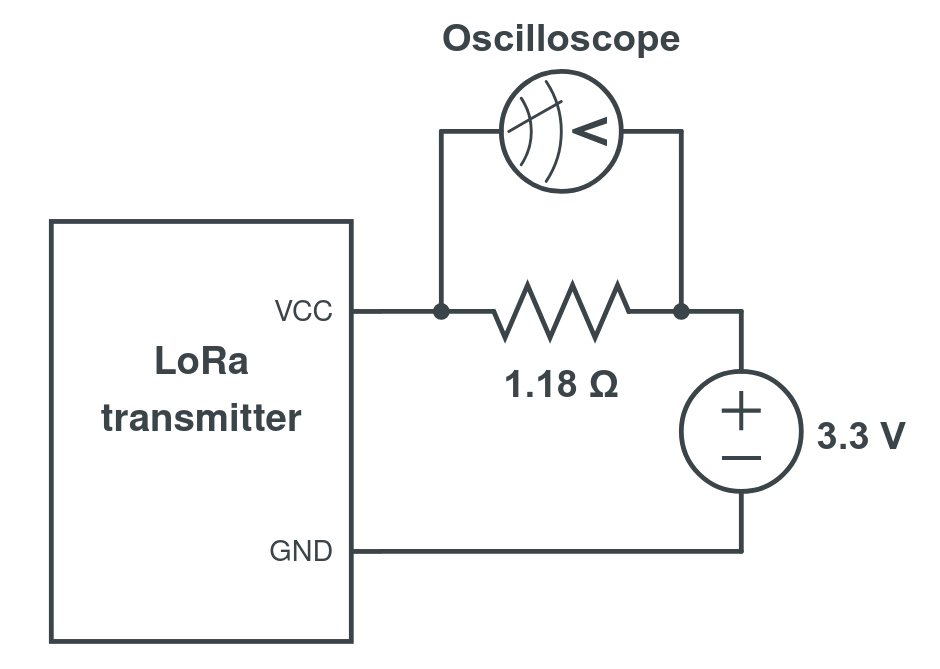
\includegraphics[width=0.5\textwidth]{images/schematic.png}\\
    \caption{Electrical diagram of the measuring setup for power draw}
    \label{img: measure setup}
\end{figure}
The tests were conducted by transmitting a single packet multiple times at identical conditions. It has been observed
that the experiment yielded exceptionally consistent results across the different transmissions. The procedure was
applied to Bacco packets and LoRaWAN packets. By analyzing the data logs collected by the oscilloscope reported in
Figure \ref{img: packet}, it is possible to measure the \gls{ToA}, equivalent to the period of time in which the board
consumed a power greater than 350 mA, and the transmission energy, equivalent to the discrete integral of the power draw
over the \gls{ToA} period. The numerical results are shown in Table \ref{tab: energy results}.

\begin{table}[ht]
    \caption{Single packet transmission numerical results.}
    \label{tab: energy results}
    \centering
    \setlength{\extrarowheight}{7pt}
    \begin{tabular}{ |c|c|c| }
        \hline
        \textbf{Parameter} & \textbf{Bacco} & \textbf{LoRaWAN}\\
        \hline
        ToA & 51.6 ms & 71.8 ms\\
        Transmission energy & 21.3 mJ & 30.8 mJ\\
        \hline
    \end{tabular}
\end{table}

\begin{figure}[ht]
    \centering
    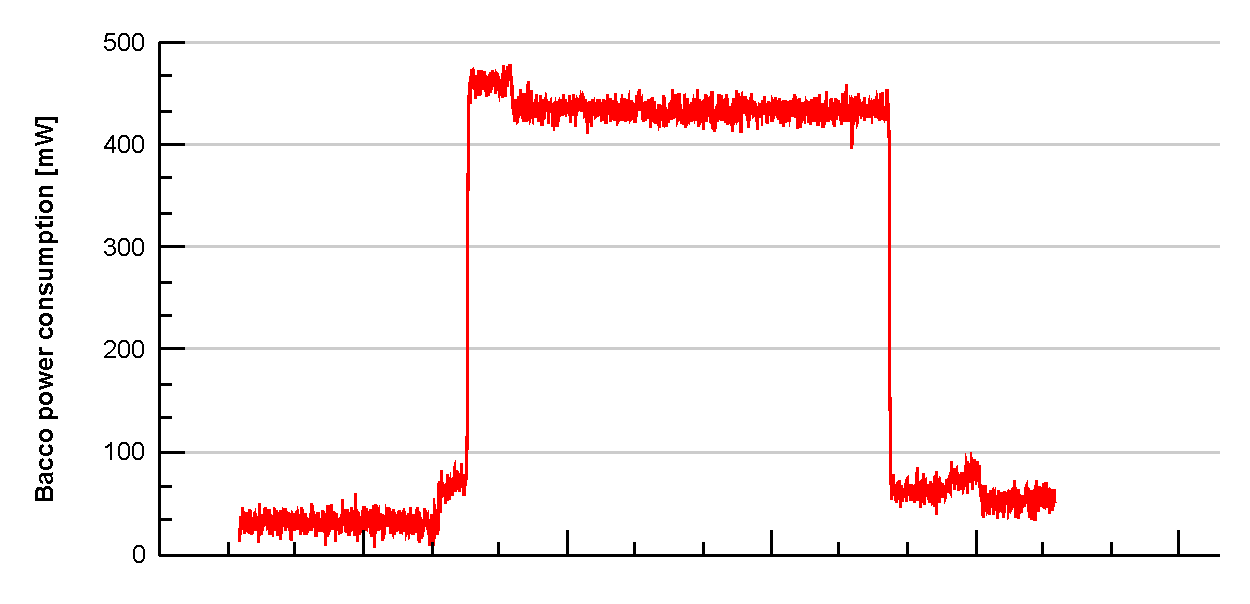
\includegraphics[width=1.0\textwidth]{images/bacco_SF7_14dbm_125khz_power.pdf}\\
    \vspace{-0.7cm}
    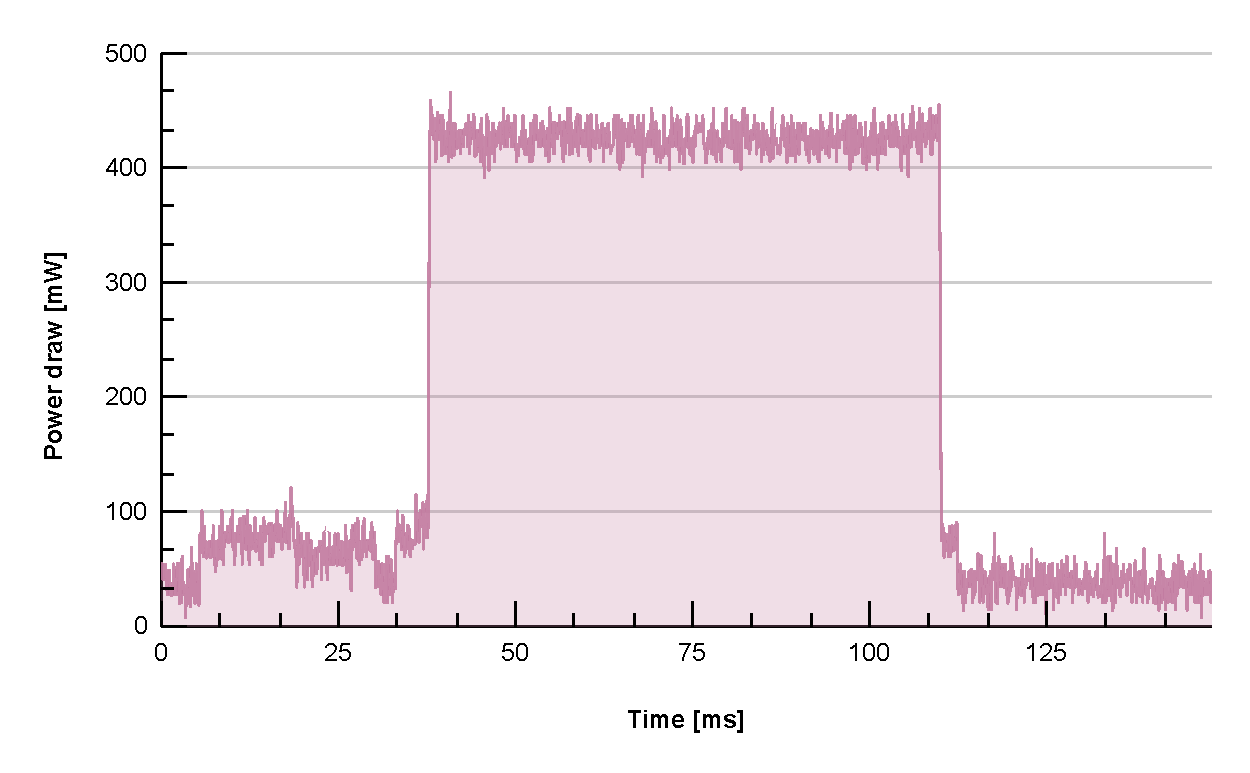
\includegraphics[width=1.0\textwidth]{images/lorawan_SF7_14dbm_125khz_power.pdf}
    \caption{Power draw of Bacco (in red) and LoRaWAN (in blue) during the transmission of a packet with a payload of 15
    bytes, using SF7, at 14dBm TX power and 125kHz bandwidth}
    \label{img: packet}
\end{figure}

\subsection{Packet Error Rate}
This section will present a test that aims to measure the packet error rate of a device transmitting messages using
Bacco. Here follows a list of the conditions under which the experiment was conducted:
\begin{itemize}
    \item \textbf{Sender nodes}: 3 x Heltec AB01 MCU, equipped with ARM Cortex M0+ Core and Semtech SX1262 LoRa module,
        see \cite{ab01}
    \item \textbf{Gateway node}: Espressif ESP32 MCU, equipped with Semtech SX1276 LoRa module
    \item \textbf{LoRa configuration}: Uplink MAC payloads with size varying between 7 and 23 bytes, spreading factor set to 7,
        output power set to 5 dBm, bandwidth set to 125 kHz.
    \item \textbf{Displacement}: The Senders were placed approximately 200 m away from the Gateway with no clear line
        of sight as they were placed in between vineyards.
    \item \textbf{Signal strength and noise}: The average \gls{RSSI} was -102 dBm and the average \gls{SNR} was 1 dBm.
    \item \textbf{Cycle time and total duration}: The transmission cycle was set to 1 hour and the experiment
        lasted a total of 2 weeks; the total number of transmitted packets was 1008.
\end{itemize}
The Gateway was programmed to count the number of successfully received packets. Table \ref{tab: error rate results}
shows the results of the experiment.
\begin{table}[ht]
    \caption{Packet error rate test results.}
    \label{tab: error rate results}
    \centering
    \setlength{\extrarowheight}{7pt}
    \begin{tabular}{ |c|c|c| }
        \hline
        \textbf{Total packets sent} & \textbf{Total packets received} & \textbf{Error rate}\\
        \hline
        1008 & 1004 & 0.4\%\\
        \hline
    \end{tabular}
\end{table}
